
%(BEGIN_QUESTION)
% Copyright 2006, Tony R. Kuphaldt, released under the Creative Commons Attribution License (v 1.0)
% This means you may do almost anything with this work of mine, so long as you give me proper credit

Beregn netto dreiemoment på trommelen fra de to viste kreftene. Trommelens ytre radius er 6 fot, og radiusen til den mindre trinsen (festet til trommelen) er 2 fot:

$$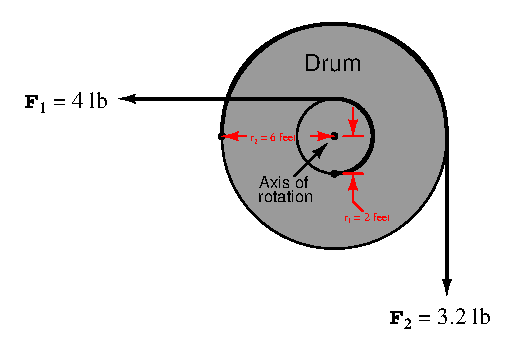
\includegraphics[width=15.5cm]{i01428x01.eps}$$

Beregn også den mekaniske fordelen i dette systemet, dersom $F_1$ regnes som {\it inngangskraften}.

\underbar{file i01428}
%(END_QUESTION)





%(BEGIN_ANSWER)

$\tau_{net}$ = 11.2 lb-ft, med urviseren
 
\vskip 10pt

$$M_A = {F_{out} \over F_{in}} = {3.2 \hbox{ lb} \over 4 \hbox{ lb}} = 0.8$$

%(END_ANSWER)





%(BEGIN_NOTES)

%INDEX% Machine, mechanical advantage
%INDEX% Physics, torque: calculation problem

%(END_NOTES)

